% THIS IS AN EXAMPLE DOCUMENT FOR VLDB 2012
% based on ACM SIGPROC-SP.TEX VERSION 2.7
% Modified by  Gerald Weber <gerald@cs.auckland.ac.nz>
% Removed the requirement to include *bbl file in here. (AhmetSacan, Sep2012)
% Fixed the equation on page 3 to prevent line overflow. (AhmetSacan, Sep2012)

\documentclass{vldb}
\usepackage{graphicx}
\usepackage{balance}  % for  \balance command ON LAST PAGE  (only there!)
\usepackage{multirow}
\usepackage{tabularx}
\usepackage{colortbl}

\definecolor{table_header}{RGB}{221,221,221}

% Include information below and uncomment for camera ready
\vldbTitle{Deferred secondary index update with LSM-trees}
\vldbAuthors{Vladislav Shpilevoy, Konstantin Osipov, Dmitry Volkanov}
\vldbDOI{https://doi.org/TBD}

\begin{document}

% ****************** TITLE ****************************************

\title{Deferred secondary index update with {\ttlit LSM-trees}}

% possible, but not really needed or used for PVLDB:
%\subtitle{[Extended Abstract]
%\titlenote{A full version of this paper is available as\textit{Author's Guide to Preparing ACM SIG Proceedings Using \LaTeX$2_\epsilon$\ and BibTeX} at \texttt{www.acm.org/eaddress.htm}}}

% ****************** AUTHORS **************************************

% You need the command \numberofauthors to handle the 'placement
% and alignment' of the authors beneath the title.
%
% For aesthetic reasons, we recommend 'three authors at a time'
% i.e. three 'name/affiliation blocks' be placed beneath the title.
%
% NOTE: You are NOT restricted in how many 'rows' of
% "name/affiliations" may appear. We just ask that you restrict
% the number of 'columns' to three.
%
% Because of the available 'opening page real-estate'
% we ask you to refrain from putting more than six authors
% (two rows with three columns) beneath the article title.
% More than six makes the first-page appear very cluttered indeed.
%
% Use the \alignauthor commands to handle the names
% and affiliations for an 'aesthetic maximum' of six authors.
% Add names, affiliations, addresses for
% the seventh etc. author(s) as the argument for the
% \additionalauthors command.
% These 'additional authors' will be output/set for you
% without further effort on your part as the last section in
% the body of your article BEFORE References or any Appendices.

\numberofauthors{3} %  in this sample file, there are a *total*
% of EIGHT authors. SIX appear on the 'first-page' (for formatting
% reasons) and the remaining two appear in the \additionalauthors section.

\author{
% You can go ahead and credit any number of authors here,
% e.g. one 'row of three' or two rows (consisting of one row of three
% and a second row of one, two or three).
%
% The command \alignauthor (no curly braces needed) should
% precede each author name, affiliation/snail-mail address and
% e-mail address. Additionally, tag each line of
% affiliation/address with \affaddr, and tag the
% e-mail address with \email.
%
% 1st. author
\alignauthor
Vladislav Shpilevoy
       \affaddr{Lomonosov Moscow State University}\\
       \email{v.shpilevoy@tarantool.org}
% 2nd. author
\alignauthor
Konstantin Osipov
       \affaddr{Tarantool}\\
       \email{kostja@tarantool.org}
% 3rd. author
\alignauthor
Dmitry Volkanov
       \affaddr{Lomonosov Moscow State University}\\
       \email{volkanov@lvk.cs.msu.su}
}
\date{24 January 2018}
% Just remember to make sure that the TOTAL number of authors
% is the number that will appear on the first page PLUS the
% number that will appear in the \additionalauthors section.

\maketitle

\begin{abstract}
Log-Structured merge-trees (LSM-trees) are becoming more and more widely
adopted as a staple data structure in secondary storage database management
systems, ending the half-a-century-long dominance of B-trees. The major
LSM-tree's advantage is that it writes new data and old data updates on disk
always sequentially. It is possible due to LSM-tree's ability to store many
versions of the same key - it allows to LSM-based tables do not read and delete
old data explicitly from primary index on such operations as deletion or replace
to delete old data. Data is deleted by new data during compaction instead. But
this advantage is nullifed by secondary indexes, because replace/delete-like
operations require read and delete old data from each secondary index explicitly.
This paper presents a modification for LSM-tree data structure, which allows to
do not read any index on replace/delete operations even if there are
non-secondary indexes in the table.
Experimental research of the modified LSM-tree shows write speed growth 1.5 to
10 times against original LSM-tree on tables with 2-4 non-unique secondary
indexes. And the more secondary indexes there are, the faster the new LSM-tree
works on write operations.
\end{abstract}

% Abstract

% -- 1. Introduction
% Краткая история появления LSM-деревьев, предпосылки к этому. Связь с SSD.
% Примеры БД. Главные преимущества (версионность, последовательность записи).
% Главный недостаток - скрытые чтения (что это). На чем проявляются
% (на обновлениях вторичных индексов), на чем нет (только на первичном), почему
% такие плохие. Сказать, что в данной статье представлен алгоритм, который
% позволяет не делать скрытых чтений на некоторых операциях по некоторым таблицам.
% В одно предложение сказать, какой прирост производительности удалось получить.

% -- 2. Background and motivation
% Более полное определение LSM-дерева. Сказать не чрезмерно подробно, какие в нем
% ключевые алгоритмы (как пишутся обновления, как делаются чтения). Сказать про
% ratio размеров уровней.
% -- 2.1. Compaction
% Сказать подробно, как делается слияние уровней, если они представлены
% сортированными массивами (вместо классического варианта, где на диске уровни -
% это B-деревья). Особо упомянуть, что старые данные дискардятся новыми только в
% пределах одинаковых ключей.
% -- 2.2. LSM-tree based index structure
% Про то, что в LSM-tree based таблицах каждый индекс - это LSM-дерево. Первичный
% индекс хранит таплы целиком, вторичный не целиком (это просто упомянуть, так как
% будть индексы хоть covering - это не помогает избавиться от скрытых чтений). Но
% важно, что вторичный индекс использует первичные ключи как ссылки на таплы в
% первичном индексе. И LSM-деревья получаются связанными.
% -- 2.3. Multiple indexes update problem
% Рассказать, что существуют delete и replace операции, которые на одном индексе
% не требуют чтений. Но при появлении вторичных индексов они делают скрытые чтения
% из первичного индекса. В случае replace вторичный ключ может поменяться, и тогда
% во вторичном индексе новая запись не удалит старую. В случае delete по
% первичному ключу есть только первичный ключ, и во вторичные индексы вставлять
% нечего - приходится тоже читать.

% -- 3. Algorithm design and implementation
% Рассказать ключевую идею алгоритма, что скрытые чтения нужны только для удаления
% старых данных, и вместо чтений сразу перед обновлением таблицы можно отложить
% эти чтения до компакта первичного индекса, когда таплы и так и эдак читаются, и
% можно сразу определить, какие таплы дискардятся. Эти таплы можно раскидывать по
% вторичным индексам как delete по вторичным ключам и версиям.
% -- 3.1 Update
% Сказать, что на апдейты более не читаем. Replace пишем сразу во все индексы.
% Delete пишем только в первичный индекс.
% -- 3.2 Compaction
% При компакте первичного индекса собираются таплы, которые собираются удалиться.
% Из них извлекаются вторичные ключи по всем вторичным индексам. Эти ключи вместе
% с версией тапла вставляются в виде delete сразу в дисковую часть каждого
% вторичного индекса. Когда вторичный индекс компактит, он учитывает эти delete,
% причем со сверкой версии - это необходимо, так как delete старых таплов попадают
% по времени во вторичный индекс позже, чем более новые данные.
% -- 3.3 Read
% Читаем как обычно. Все чтения лукапят в первичный индекс. Если там тапл не
% найден, то он пропускается и вторичный индекс читается дальше в соответствии с
% тем, какой был запрос пользователя.
% -- 3.4 Implementaion
% Реализация выполнена на основе БД Tarantool и ее движка Vinyl, который хранит
% данные в LSM-деревьях по ренжам. Ядро нового алгоритма сосредоточено в
% процедуре компакта уровней, где из старых таплов извлекаются вторичные ключи и
% версии, и вставляются сразу на первый уровень (считая с нуля) LSM-деревьев
% вторичных индексов. Пересортировка удаляемых данных первичного индекса в
% порядок вторичных индексов выполняется в памяти по мере чтения схлопываемых
% уровней первичного индекса.

% -- 4. Mathematical basics
% Привести формулы в двух группах: ДО патча и ПОСЛЕ. В каждой группе вывести
% сложность replace, delete, primary get. Учесть level_size_ratio, "ветвистость"
% деревьев в памяти, кол-во таплов в памяти, кол-во уровней на диске и размер
% первого уровня (считая с нуля) первичного индекса.

% -- 5. Evaluation
% Сказать, что наибольший прирост получается при replace/delte операциях и
% зависит, согласно формулам выше, от размеров индексов, ratio и прочего. И что
% кроме наилучшего случая рассмотрен Linkbench. (Постараться сделать сравнения
% не только Тарантула с собой, но и с LevelDB и с MySQL (MyRocks)).
% -- 5.1. Microbench
% Тут показать волшебный прирост 10х, сказать на чем. И сделать такой же тест для
% MyRocks и LevelDB (они усосут, но надо понять, насколько - может еще больше).
% -- 5.2. Linkbench
% Тут показать результаты, которых пока нет, против тех же БД. Ожидается, что
% прирост будет не сказать, что сильно велик, так как там много чтений (явных).

% -- 6. Related work
% Рассказать, что кроме нового алгоритма есть еще куча старых, даже для
% B-деревьев. Чуть-чуть про них рассказать.
% -- 7. Conclusion
% Сказать, что новый алгоритм воскрешает версионность LSM-таблиц со множеством
% индексов. И что можно оптимизировать. Например, при дампе вторичных индексов
% лукапить первичный, чтобы проверять, что какие-то таплы уже может можно и не
% дампить. И помечать такие таплы на диске в первичном индексе, чтобы они при
% удалении во время компакта не создавали делитов.
% И что можно сократить расход памяти во время пересортировки до константного,
% если сделать сортировку слияниями кучки файликов, которые будут копиться во
% время компакта.
% -- 8. References


\section{Introduction}
Log-Structured Merge trees were developed for write-intensive tasks in 1990th
and were used in file systems and for reserve copying. But their prevalence was
restricted by hidden reads.

These are the reads which accompany writes: e.g. when it’s necessary to delete
old data from a secondary index after an update, or check an unique or a foreign
key constraint. A significant amount of reads in a modern database is hidden.
Such reads, when followed by a write, cost nearly nothing in a B-tree, but can
penalize performance of an LSM-tree based table to an extent when its write
advantage becomes completely diluted.

With Solid-State Drive (SSD) appearance cost of random writes had started
contribute to overall performance way more heavily than cost of random reads,
and nowadays the LSM-tree is consideted to be a standard data structure for
databases. For example, it is used in LevelDB, RocksDB, Cassandra, Tarantool,
BigTable, Hbase, Riak, MySQL (MyRocks).

However SSD does not help in a special case, which is very popular and dilutes
LSM-tree's ability to store multiple versions of the same keys. It is linked
with LSM-tree compaction algorithm, and appears on tables with multiple indexes.

In a primary LSM-tree based index any replace or delete operation is executed
with no hidden reads because of LSM-tree ability to store multiple key versions.
A new tuple is just inserted into memory and after some compactions discards old
tuples. But it is not possible if there are secondary indexes. If a table
contains secondary indexes, any update operation must read an old tuple from a
primary index, extract from it secondary keys and delete them from each
secondary index explictly. That is any update of such table produces hidden
reads from a primary index.

Primary index read and explicit old tuple deletion can not be avoided in classic
LSM-tree, because it deletes old versions of the key only if these versions are
equal by the key. If a request changes a secondary key in an exising tuple and
does not deletes old one, then it is not deleted from a secondary index.
LSM-tree considers new and old tuple not to be different versions of the same
key, but to be different keys.

The paper describes a new LSM-tree compaction algorithm, a new LSM-tree based
table update and read algorithms. Replace and delete operations on the new
LSM-tree do not any reads regardless of secondary index number, if all of them
are not unique. Experiments show exponential requests number per second (RPS)
grow on some loading types and some schemas. For example, on a table with 3
non-unique secondary indexes and replace/delete batched requests RPS increased
up to 10 times.

\section{Background and motivation}
This section defines some LSM-tree basics: how it is can be stored on disk and
in memory, how compaction, update and read works. What LSM-tree parameters are
typically configurable.

LSM-tree is a data structure optimized for write-intensive tasks. It has
multiple levels: zero-level is stored in a memory and other on a disk.
Zero-level amasses updates and periodically is dumped on to a disk to become
first level. Zero-level after dump are cleaned up and collects new updates. And
so on.

Zero-level usage allows to write updates to a disk in batches regardless of
their order, keys, types. Even delete is put in a zero-level as a tuple of a
special type.

When level number became too big, the LSM-tree is compacted - several levels are
merged in a new one. During compaction new tuples discard old tuples of the same
key. For example, delete discards all older data and sometimes itself; replace
discards all older data, but not itself.

LSM-tree can store levels in multiple ways. For example, memory level can be
B-tree or Red-Black tree. Disk levels can be organized as B-trees or sorted
arrays. In the paper sorted arrays on disk and B+ tree in memory are considered.

\subsection{Compaction}
\begin{figure}
\centering
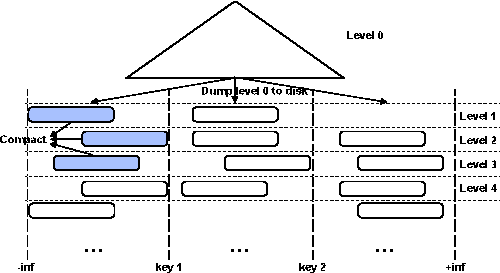
\includegraphics[width=0.4\textwidth]{compaction_schema}
\caption{LSM-tree ranges dump and compaction}
\label{fig:compaction_schema}
\end{figure}
Each level consists of multiple sublevels. Each sublevel is an array sorted by
a key (in a case of LSM-tree index the key consists of index parts) and
containig a specific key values range. During compaction some sublevels of each
levels are merge-sorted into a new sorted array. It is known, that if one key
version is on level $i$ and another on $j < i$, then the key version on level
$j$ is newer and another one is discarded when compacted.

Compaction procecure is needed to reduce level count and to discard old tuples
to make room for new ones. Compaction frequency is regulated by LSM-tree
parameters level size ratio and maximal sublevels count. In each pair of
neighbour levels $i$ and $i + 1$ size of a level $i + 1$ must be greater than
level $i$ size $*$ level size ratio at least. If maximal sublevels count per
level is exceeded or level size ratio is violated, then compaction procedure
merges as much sublevels as needed to satisfy both limitations.

In practice, sublevels are produced by memory level dump and by spliting index
key values into ranges, when each range stores and maintains its own sublevels
independently of other ranges (see Figure \ref{fig:compaction_schema}).

\subsection{LSM-tree based table structure}
In LSM-tree based table each index is an LSM-tree, sorted by the index parts.
It is common pattern, that a table has one primary index and a number of
secondary indexes. A primary index always is unique, and stores full tuples,
including all indexed and not indexed fields, as they were inserted by an user.
A secondary index stores only its own key parts and primary index parts to save
memory. Such indexes are called non-covering. Primary parts are used as link to
a full tuple in a primary index, when a search uses a secondary index only.

The described pattern is not unique feature of LSM-tree based tables. For
example, SQLite secondary indexes based on B-tree are not covering by default
too. And each SQLite table has unique primary index even if an user did not
specified it explicitly.

Since secondary indexes stores primary index parts, they are linked with primary
indexes. And if a tuple does not exist in a primary index, the same tuple can
not exist in a secondary index. This is the reason, why hidden reads are
indispensible - if a tuple is replaced with another secondary key or deleted
from a primary index, then its old version must be deleted from each secondary
index by old secondary key, else a table indexes are not consistent.

\subsection{Multiple indexes update problem}
LSM-tree ability to manage multiple versions of a key allows to avoid hidden
reads on such operations as replace or delete which can not break consistency if
there is only a primary index in a table and no foreign key constraints.
Such operations are known as \textbf{blind-writes} \cite{kai:slimdb}.
Blind-writes are much faster than non-blind insert or update operations, which
read an old tuple in a worst case from a disk to check for duplicate or apply
update operations.

The big problem of LSM-tree based tables is that in presense of secondary
indexes all writes become non-blind. See Figure \ref{fig:inconsistent_example}
for example of inconsistency if replace is blind and a table has secondary
index. Here a table is defined with 4 columns: first is part of a primary index,
2 and 3 are parts of a secondary index, and 4 is not indexed.
\textit{Replace\{1, 5, 6, 7\}} before executed must read old tuple from a
primary index by the key \textit{\{1\}}, extract the secondary key
\textit{\{2, 3\}}, delete it from the secondary index, and only then insert the
new tuple. If the old tuple is not deleted, then during compaction it becames
garbage with no link to a full tuple in the primary index.
\begin{figure}
\centering
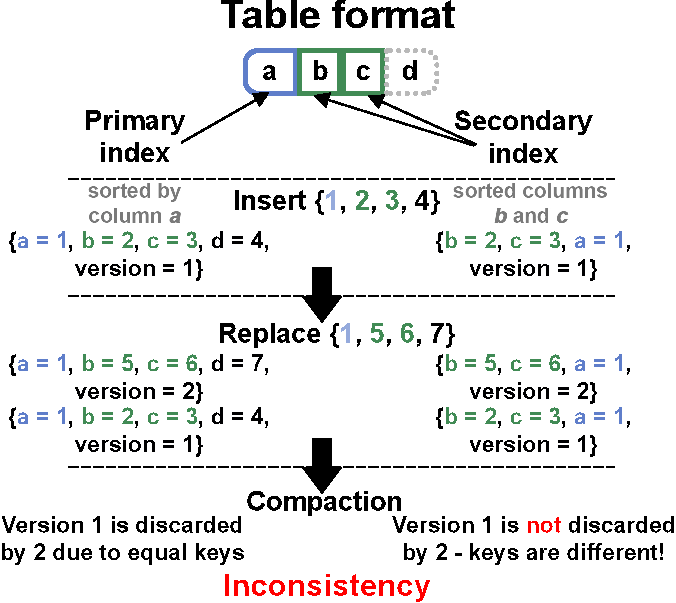
\includegraphics[width=0.3\textwidth]{inconsistent_example}
\caption{LSM-tree based table inconsistency example}
\label{fig:inconsistent_example}
\end{figure}

Since disk access is much slower than memory access, secondary index presence
destroys LSM-tree versions advantage. In the next section a new LSM-tree update
algorithm is presented reviving versions and blind-writes.

\section{Design and implementation}
Below the basics of a new algorithm are described, followed by three sections,
each of which unfolds one of enclosed part of the algorithm.

The key idea of the algorithm is that deletion of old data can be deferred until
primary index compaction stage. It allows to do not hidden reads during replace
and delete by primary key operations since they use hidden reads only to learn
and delete old secondary key versions, not to check consistency. It works on
tables with non-unique secondary indexes only, because it is impossible to break
consistency of non-unique secondary index using delete or replace operations.

Obviously, it is not true if there are unique secondary indexes. For example,
consider a table with columns \textit{\{a, b\}}, unique primary index on
\textit{\{a\}} and unique secondary index on \textit{\{b\}}. A table contains
two records: \textit{\{1, 1\}} and \textit{\{2, 2\}}. It is impossible now to do
replace \textit{\{1, 2\}}, because it leads to duplicate in the secondary index.

Of course, in MySQL, for example, replace would delete both old records, but
such kind of replace can not be deferred because during the primary index
compaction there is no way to learn that a new tuple with one primary key
discards an old tuple with another primary key without explicitly inserted
deletion. This multi-replace must delete old records with another primary keys,
and it is not considered under the paper.

The algorithm of deferred update consists of three enclosed parts:
\begin{enumerate}
\item Update of a zero-level of all indexes. This is where replace and delete by
a primary key are inserted into memory and makes secondary and primary indexes
mal-synchronized.
\item Compaction, which differs in primary and secondary indexes. A primary
index during compaction detects tuples to discard and sends them to a secondary
indexes as a new LSM-tree sublevel. A secondary index on compaction takes into
account sublevels received from a primary index.
\item Secondary index reading, that now can see tuples already deleted from a
primary index. Existance of a concrete version of a key read from a secondary
index must be check via primary index lookup.
\end{enumerate}

\subsection{Deferred update}
Only two operations can be deferred: replace and delete by a primary key. At
first algorithm of replace execution is presented, and then the delete's one
which is very similar.

Consider a table with one primary index and some non-unique secondary indexes.
Assume an user executes replace. A tuple specified in the replace is inserted
into each indexe's memory level as is, with no preliminary reading and deletion
of an old tuple from secondary indexes.
\begin{figure}
\centering
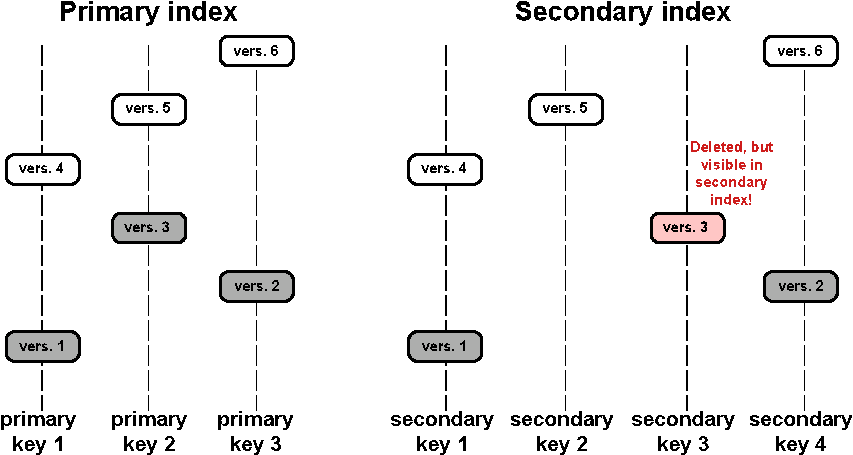
\includegraphics[width=0.46\textwidth]{table_after_deferred_update}
\caption{LSM-tree based table if update is deferred}
\label{fig:table_after_deferred_update}
\end{figure}

When this algorithm is used, it is possible and valid, that some secondary
indexes consider discarded tuples as not discarded, like in example on Figure
\ref{fig:table_after_deferred_update}. In the example there is a tuple with
version 3, which is discarded in a primary index by a newer tuple with the same
key and version 5. But secondary keys of these tuples are different, and a
secondary index sees the tuple with version 3 as a separate non-discarded tuple.
Such tuples, visible in a secondary index and not visible in a primary one are
called \textbf{dirty}.

A delete by a primary key is inserted only in a primary index memory. It can not
be inserted in a secondary index, because a corresponding secondary key is
unknown with no hidden reads. In such a case a tuple, discarded by the delete,
becomes dirty in each secondary index.

In the next section the algorithm of deletion of dirty tuples is presented as a
part of new LSM-tree compaction procedure.

\subsection{Compaction}
\subsubsection{Primary index}

Compaction is triggered by the same signals, as in the classic LSM-tree - by
too big number of sublevels, or too big difference in neighbour levels size.

Consider the basic compaction, when there are no deferred updates and dirty
tuples. Assume the levels consist of sublevels belong to key ranges, and a
sublevel is sorted array of versioned keys.

Sublevels are compacted in merge-sorting procedure discarding tuples having
older versions among compacting sublevels. That is if a tuple has newer version
out of compaction participants, then it is not discarded. Two tuples are
considered to be verions of the same key, if they are equal by parts of
compacting LSM-tree index. If compaction participants have several versions of a
key then during merge-sort they met during one of merge-steps, and only one
tuple stays. After merge-sort is finished, a new single sublevel replaces old
ones.

Obviously, old tuples are read from disk during compaction. And these reads
replace hidden reads of update operations. Actually, the hidden reads are
deferred until compaction, where they are done anyway and sequentialy -
sequential read is at a far quicker than random both on SSD and HDD.

Old tuples going to be discarded are used to extract dirty secondary keys.
Extracted keys are resorted into order of a secondary index, and are written as
a new sublevel directly into the secondary index. Secondary keys are written as
deletes saving the version of the original tuple. New primary index compaction
produces subleves for itself and for each secondary index. When a secondary
index compacting, it takes into account sublevels, created for it by a primary
index.

Resorting into order of a secondary index is executed to observe LSM-tree
indexe's invariant whereby sublevel of an index is an array tuples sorted by key
parts of the index. So sublevels, created for secondary indexes during primary
one's compaction, must be resorted into secondary index order. Resorting method
depends on implementation, and can be
\begin{itemize}
\item in-memory quick sort after all tuples are read from disk;
\item in-memory tree-sort, when for each index a tree is created before
compaction and it is filled just as tuples are reading from disk. Tree can be of
any type: binary, red-black, B-tree. When a primary compaction is finished, the
tree is written into a secondary index sublevel as a sorted array. So such a
tree is prefered, which can be iterated fast over all keys
(B\textsuperscript{+}-tree for example - it maintains sorted list of stored
values);
\item disk merge-sort, which can be used when sublevels compaction discard too
many tuples and there are many secondary indexes - they may no fit into memory.
The idea is to do in-memory sort of discarded tuples by batches of some fixed
size, and dump them as sorted arrays into temporary files. When the primary
compaction is finished, the congested temporary sorted arrays are merge sorted
into single sublevel intended for a secondary index. Merge-sort of temporary
files is executed in the same way as sublevels compaction - read and write files
in parts with no reading them all into memory. The described procedure is
executed for each secondary index.
\end{itemize}

\subsubsection{Secondary index}

Compaction procedure of a secondary index is slightly changed to correctly
process the deletes received from a primary index. The point is that the
deletes, received from a primary index, have both the same version and the same
key as the dirty tuples, for which they are intended, and a compaction procedure
must correctly process these versions and keys match.

The only modification of a secondary index compaction is that in a case of
versions and keys match of delete and replace tuples the replace tuple must be
discarded, and the delete tuple must stay, if it is not \textbf{major}
compaction. A compaction is major, if all sublevels of all levels are compacted.
\begin{figure}
\centering
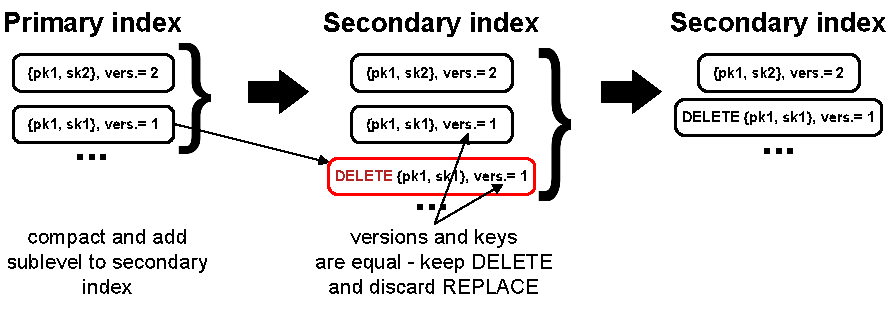
\includegraphics[width=0.46\textwidth]{secondary_compaction_example}
\caption{Secondary index compaction example}
\label{fig:secondary_compaction_example}
\end{figure}
On the Figure \ref{fig:secondary_compaction_example} it is presented example of
a secondary index compaction with sublevel, received from a primary index.
In the example, a primary and secondary indexes stores two tuples:
\textit{\{pk1, sk1\}} and \textit{\{pk1, sk2\}}. In a primary index it is the
different versions of the key \textit{pk1}. When a primary index is compacted,
a tuple \textit{\{pk1, sk1\}} is discarded and sent to a secondary index as a
DELETE tuple with the same version. During a secondary index compaction this
DELETE \textit{\{pk1, sk1\}} with version 1 mets the dirty tuple
\textit{\{pk1, sk1\}} with version 1 - their keys and versions are equal. It is
assumed, that it is not major compaction, so the tuple \textit{\{pk1, sk1\}} is
discarded and the DELETE tuple stays.

\subsection{Read}

Read of a primary index is not changed, because dirty tuples can appear in
secondary indexes only. When a secondary index is read, the dirty tuples are
skipped. To check a tuple if it is dirty, its primary key and version are looked
up in a primary index. If a primary index contains the same key with the same
version, then the tuple is not dirty and can be returned to an user.

It means, that even point reading from a secondary index can lead to multiple
lookups in a primary index to exclude dirty tuples.
\begin{figure}
\centering
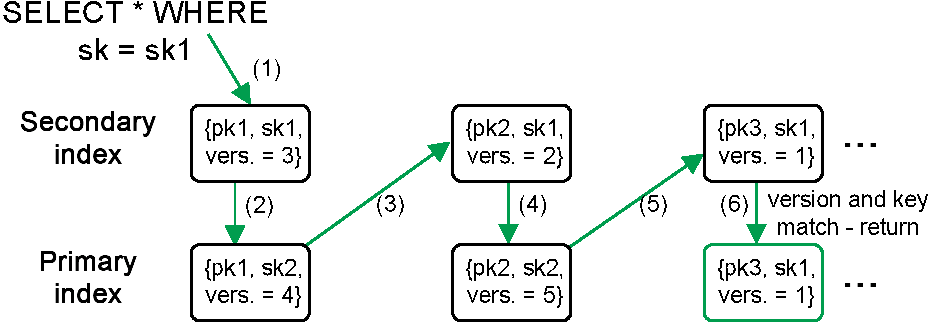
\includegraphics[width=0.46\textwidth]{secondary_reading_example}
\caption{Secondary index read example}
\label{fig:secondary_reading_example}
\end{figure}
On the Figure \ref{fig:secondary_reading_example} a SELECT by a secondary key
returns a tuple on a third attempt. At first, it reads \textit{\{pk1, sk1\}} as
the newest known version of this secondary key. It appers to be dirty, because
in a primary index a tuple with the same primary key has another version and
another secondary key. At second \textit{\{pk2, sk1\}} is checked as the next
by version: it is dirty too - in the primary index this tuple is already
replaced by \textit{\{pk2, sk2\}}. At third \textit{\{pk3, sk1\}} is checked,
and in the primary index a tuple is found with the same key and the same
version - it means, that this tuple is not dirty and can be returned to an user.

The common algorithm is to read secondary index tuples and lookup each one in a
primary index until their versions and keys match.

\subsection{Implementation}

The developed algorithm is implemented as a patch for Tarantool database's disk
engine named Vinyl. Tarantool is DBMS and application server, which supports two
storage engines: Memtx in memory and Vinyl on disk. Tables in Tarantool are
being called \textit{spaces}. Memtx engine stores data in memory in
B\textsuperscript{+}-trees, and it is not considered here.

Vinyl engine stores indexes as LSM-trees. LSM-tree based index is split into key
ranges. LSM-tree level consists of sublevels, produced by zero-level dump and
compactions. Sublevels are files. Ranges are compacted independently of each
other. Dump and compaction are executed in background threads, while transaction
processing is in a single main thread and it does not heavy operations like disk
or network access - it delegates these tasks to worker threads.

Sublevels consists of pages. Page knows its minimal and maximal keys and minimal
and maximal versions - this information is stored in memory and allows to
read just needed pages, not entire sublevels. Page size is configurable, and the
greater it is, the smaller meta info stored in memory and the bigger chunks are
read when searching for a key.

Each vinyl sublevel has bloom filter with several improvements: less hashing
with the same performance \cite{Kirsch:bloom_less_hashing} and blocked bloom
filters \cite{Putze:bloom_cache_oblivious}.

Main thread consists of coroutins written in C and called \textit{fibers}. When
a main thread wants to do long operation like LSM-tree index dump or compaction,
access disk or network, it sends a request to a worker thread and switches to
another fiber, while the original one waits for response from the worker. The
big advantage of such schema, that there are no locks on internals except
inter-thread communication queues.

Implementation of the deferred update algorithm consists of three parts like the
algorithm itself: new replace and delete execution, compaction and read.

New replace/delete are quire simple: they just do not hidden reads. Replace is
inserted in zero-levels of all indexes of Vinyl space, delete is inserted into a
primary one only.

The compaction is the most complex part of the implementation. As applied to
Vinyl and LSM-trees, the compaction procedure works as follows before the
deferred update:
\begin{enumerate}
\item Main thread detects that a compaction is necessary (for example, level
size ratio is violated or a level consists of too many sublevels), and sends a
request to a worker thread with information, which sublevels need to compact, in
which files they are stored;
\item Worker thread sees request and starts compaction. Compaction is executed
using merge-sort of sublevels files. Processed files are not deleted or changed
by a worker thread, because they may be used now in the main thread for reads.
When the worker has finished the work, it has one new sublevel file. The main
thread is notified, that the work is done;
\item After a while, one of fibers of the main thread sees the finished worker,
gets the new sublevel, puts it in the LSM-tree and deletes old sublevels and
their files atomically.
\end{enumerate}

\begin{figure}
\centering
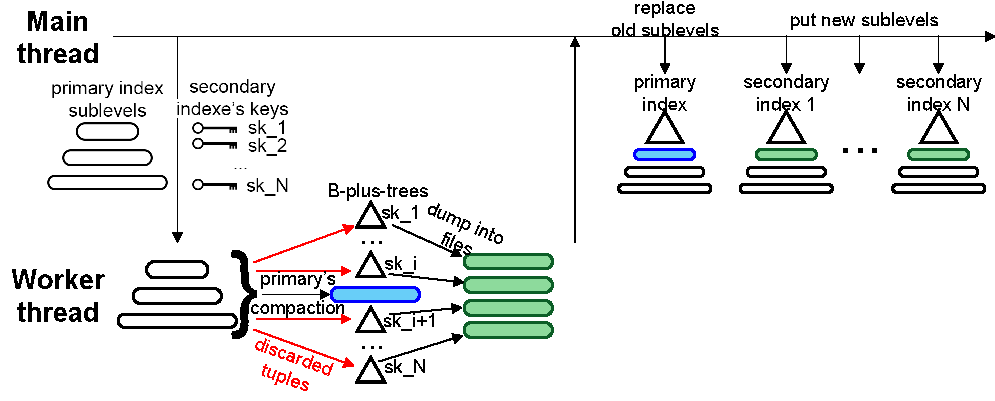
\includegraphics[width=0.46\textwidth]{compaction_implementation}
\caption{Primary index compaction schema}
\label{fig:compaction_implementation}
\end{figure}
After the deferred update is applied, the compaction procedure's second and
third steps are completely different. See Figure
\ref{fig:compaction_implementation} as illustration. When a primary index is
scheduled for compaction, the main thread sends to a worker info not only about
a primary indexe's sublevel, but about each secondary index key parts. They are
needed to extract secondary keys from primary index tuples.

While the primary index is being merge-sorted, discarded tuples are stored into
in-memory B\textsuperscript{+}-trees created for each secondary index. When a
primary index compaction is finished and a new sublevel is created, the filled
B\textsuperscript{+}-trees are dumped into sublevel files for secondary indexes.
The dump is fast, because B\textsuperscript{+}-tree can be fast iterated due to
links between neighbour keys. At this step the worker thread has sublevel files
for each index of the table, and it notifies the main thread about the finished
work.

One of the main thread's fiber replaces compacted sublevels with a new one in a
primary index, and puts secondary indexe's sublevels into corresponding indexes
at the LSM-tree's first level. Secondary index sublevel received from a primary
index is on the LSM-tree's first level, because it can contain any DELETEs from
first to last primary index levels and it means, that it can overlap any
sublevel stored on disk. These DELETEs must overlap dirty tuples for which
intended.

Implementation of reading is changed to take into account dirty tuples
existence. There is the same point that during a secondary index compaction -
the index contains both dirty tuples and their DELETEs with the same key and
version. If an iterator sees this match, it skips these versions and all olders.
All other found tuples are looked up in a primary index. If in the primary index
the tuple is found with the same secondary key and version, as the tuple from
the secondary index, then this tuple is not dirty and can be returned to an
user. Else the tuple is dirty - its DELETE while is not generated by primary
index compaction. The salient feature of this implementation that sublevels,
received from a primary index, are undistinguishable from usual sublevels, and
they are beeing read together with others. It allows to avoid lookup in a
primary index, if a tuple is dirty and its DELETE already is in the secondary
index. But there is overhead for reading these additional sublevels.

There is another way to implement reading, which has its own benefits and
drawbacks. The key concept is to distinguish sublevels received from a primary
index from others and use them for compaction only, not for reading. It allows
to read less sublevel files, but compels to do lookups in a primary index on
each tuple even if the dirty tuple's DELETE is already received from the primary
index.

\section{Mathematical basics}

In this section the mathematical complexity of original update algorithm is
compared against the deferred one's. There are used the following known values:
\begin{align*}
N &- \text{tuples number on all levels}, \\
b &- \text{zero-level B\textsuperscript{+}-tree branching factor}, \\
r &- \text{level size ratio}, \\
K &- \text{total indexes number}.
\end{align*}

According to LSM-tree level size ratio definition, level $i$ is $r$ times
bigger, than $i - 1$, so total count of levels is $O(log_rN)$
\cite{kai:slimdb}. Lets denote it as $lc$.

Deferred update algorithm allows to do not reads, but it puts new tuples in
memory level, and it is the only common part of old and new algorithms. Memory
level access complexity depends on tuples number, which can be calculated from
$N$ and levels number. Denoting memory (alias zero) level size as $m$, calculate
it via geometrical progression sum formula:
\begin{gather*}
N = m + m*r + m*r^2 + ... + m*r^{lc}, \\
N = \frac{m(1 - r^{lc+1})}{1 - lc}, \\
m = \frac{N(1 - r)}{1 - r^{lc + 1}}.
\end{gather*}

In the scope of the paper, memory level is B\textsuperscript{+}-tree, in which
search and insertion complexity is $O(log_bm)$.
Total complexity of replace and delete before deferred update includes point
search on disk - complexity of this operation is $O(log_rN)$. It is associated
with levels number because disk index of levels (pages, their minimal and
maximal keys, versions) is stored in memory and needed pages on a disk for a
certain key can be found with no disk access. Disk is accessed only to read
pages, which can contain a sought key.

Using found parameters, the complexity of update can be calculated:

\underline{Complexity of replace}:
\begin{displaymath}
O(log_bm) + O(log_r(N - m)) + O(log_bm) * (2K - 1)
\end{displaymath}
Do hidden read: scan for an old tuple in memory level ($O(log_bm)$), on
disk ($O(log_r(N - m))$). In the worst case an old tuple with the same primary
key is found, so insert into memory level ($O(log_bm)$) of each secondary index
two tuples ($2(K - 1)$): DELETE of the old one and the new tuple. In the primary
index the new tuple discards the old one without DELETE, so in the primary
index only one tuple is inserted ($2(K - 1) + 1 = 2K - 1$).

\underline{Complexity of delete}:
\begin{displaymath}
O(log_bm) + O(log_r(N - m)) + O(log_bm) * K
\end{displaymath}
Do hidden read: scan for an old tuple in the primary index disk and memory
($O(log_bm) + O(log_r(N - m))$). In the worst case an old tuple is found -
insert into memory level of each index DELETE tuple ($O(log_bm) * K$).

After the deferred update is implemented all hidden reads disappear.

\underline{Complexity of \textbf{deferred} replace}:
\begin{displaymath}
O(log_bm) * K
\end{displaymath}
Simply insert a new tuple into memory levels of all indexes - no DELETEs, no
hidden reads. They are deferred until compaction. The deferred replace is at
least twice faster than classical one according to the calculations below:
\begin{gather*}
\frac{O(log_bm) + O(log_r(N - m)) + O(log_bm) * (2K - 1)}{O(log_bm) * K} = \\
\frac{O(log_bm * 2K) + O(log_r(N - m))}{O(log_bm) * K} = \\
2 + \frac{O(log_r(N - m))}{O(log_bm) * K}.
\end{gather*}
LSM-trees zero level size is bounded above by RAM size, indexes number is set
once when a database schema is created and is changed rare, zero-level
B\textsuperscript{+}-tree's branching factor is constant, so the nominator
$O(log_bm) * K$ can be treatted as constant. Denominator contains $N$, which
in write-intensive tasks can be huge (billions and more) and the bigger it is
the bigger is the difference between speed of deferred and simple update.
For example, for the following estimation:
\begin{align*}
&r = 3, \\
&b = 10, \\
&m = 10^5, \\
&N = 10^8, \\
&K = 5.
\end{align*}
the deferred replace is faster in $~2.55$ times in theory. In the reality the
speed growth is much and much greater, because access to disk is much slower
than access to memory even for SSD. And exactly on disk speed depends the
denominator $O(log_r(N - m))$ - when $N$ is big, most of tuples are stored on
disk. It is because it is easy to get speed growth up to 10 times even on small
tables.

\underline{Complexity of \textbf{deferred} delete}:
\begin{displaymath}
O(log_bm)
\end{displaymath}
Insert DELETE into primary indexe's memory level only. Because only primary
index is used, the deferred delete is faster than the simple in at least $K + 1$
times, and the more tuples are on disk, the faster deferred delete is:
\begin{gather*}
\frac{O(log_bm) + O(log_r(N-m)) + O(log_bm) * K}{O(log_bm)} = \\
\frac{O(log_bm)*(K + 1) + O(log_r(N-m))}{O(log_bm)} = \\
K + 1 + \frac{O(log_r(N-m))}{O(log_bm)}
\end{gather*}

\section{Evaluation}

The implemented algorithm is tested on two benchmarks: microbench, on which the
difference between usual and deferred update are most significant, and
linkbench. Both benchmarks are done on a single machine with Apple SSD SM0512L,
Intel i7 2.7Ghz, 4 cores.

\subsection{Microbench}

The benchmark compares stock Tarantool vs Tarantool with deferred updates.
Obviously, the biggest throughput improve can be achieved on workload consisting
of many replaces and deletions to a table with non-unique secondary indexes.
The database schema consists of one space on Vinyl engine, one primary index on
a first field, and 4 secondary indexes each on a one field. In SQL syntax:
\begin{verbatim}
create table test (field1 unsigned integer primary key, field2 unsigned integer,
		   field3 unsigned integer, field4 unsigned integer,
		   field5 unsigned integer);
create not unique index on test(field2);
create not unique index on test(field3);
create not unique index on test(field4);
create not unique index on test(field5);
\end{verbatim}

\begin{figure}
\centering
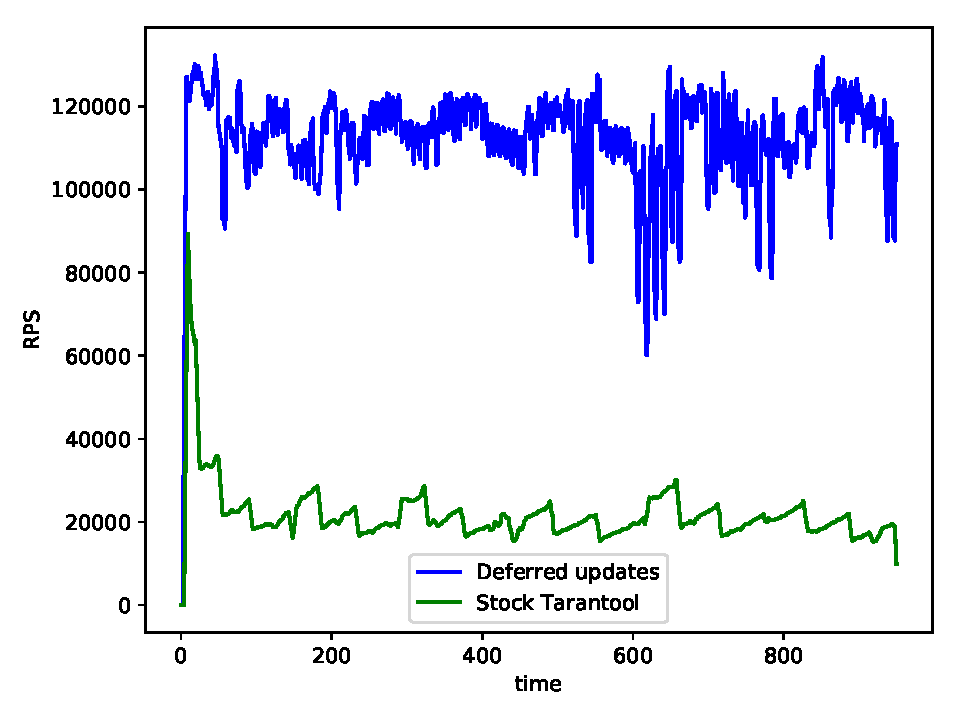
\includegraphics[width=0.46\textwidth]{rps_microbench}
\caption{Microbenchmark RPS}
\label{fig:microbench}
\end{figure}

LSM-tree's zero-level size is restricted with 128Mb. Workload is generated and
sent via network by 4 clients on the same machine as Tarantool (unix sockets are
used - overhead of network is minimal). Each client generates replaces and
deletions by primary key in batches with randmo size 1 to 500 tuples. Half of
tuples are deletions and half are replaces. A tuple consists of 5 fields with
total size about 50 bytes (including tuple meta info). All keys are between 1
and 1000000.

There are two worker threads to dump and compact levels. Level size ratio is
3.5, maximal sublevels count on a level is 2, bloom filter has 5\% false
positive rate, page size is 8Kb (about 160 tuples capacity).

The results are on Figure \ref{fig:microbench}.

There are some aggregated characteristics in Table \ref{table:rps_microbench}.
\begin{table}
\centering
\caption{Microbenchmark RPS aggregated}
\label{table:rps_microbench}
\begin{tabular}{|c|c|c|} \hline
\cellcolor{table_header}&
\cellcolor{table_header}Deferred update &
\cellcolor{table_header}Simple update\\ \hline

\cellcolor{table_header}Average &112343 r/s &21681 r/s\\ \hline
\cellcolor{table_header}Maximal &132316 r/s &89292 r/s\\ \hline
\cellcolor{table_header}Median &114772 r/s &20097 r/s\\
\hline\end{tabular}
\end{table}

\subsection{Linkbench}

\section{Related work}
Necessity to speed updates up is not a new task. There are some existing works
on this theme: some of them try to reduce hidden reads number, another try to
defer some computations until reads. Various decisions are developed not for
LSM-trees only for for B-trees too.

The problem of too long updates appeared earlier than SSD disks, when B-trees
was the very widespread data structure for HDDs. In the work
\cite{Edward:incremental_update} authors propose a method of deferring updates
of B-tree until updated keys are read. Updates are stored in
\textit{differential files}, which are used firtly to lookup each key.
Differential files were first proposed in 1976 \cite{Lohman:differential_files}
as a method of B-tree multiversion support. It is curious that LSM-tree
investigated much later actually completely consists of differential files.
Differential files allowed to store multiple versions, but they could not reduce
cost of random read-writes in B-trees.

In 2014 another optimization of LSM-tree performance was proposed
\cite{Wang:open_channel_ssd} on a hardware level. According to this paper, SSDs
do not allow fully utilize I/O performance because of providing only one channel
to an operating system even if SSD has multiple channels, which can be accessed
simultaneously. On the base of custom LevelDB, it was showed, that usage of
open-channel SSD (SDF) allows to improve throughput in more than 4 times. But
this optimization is actually hardware, and the LSM-tree is not changed, so on
simple SSDs it does not work. But this method can be combined with deferred
updates.

\subsection{Tables}
Because tables cannot be split across pages, the best
placement for them is typically the top of the page
nearest their initial cite.  To
ensure this proper ``floating'' placement of tables, use the
environment \textbf{table} to enclose the table's contents and
the table caption.  The contents of the table itself must go
in the \textbf{tabular} environment, to
be aligned properly in rows and columns, with the desired
horizontal and vertical rules.  Again, detailed instructions
on \textbf{tabular} material
is found in the \textit{\LaTeX\ User's Guide}.

Immediately following this sentence is the point at which
Table 1 is included in the input file; compare the
placement of the table here with the table in the printed
dvi output of this document.

\begin{table}
\centering
\caption{Frequency of Special Characters}
\begin{tabular}{|c|c|l|} \hline
Non-English or Math&Frequency&Comments\\ \hline
\O & 1 in 1,000& For Swedish names\\ \hline
$\pi$ & 1 in 5& Common in math\\ \hline
\$ & 4 in 5 & Used in business\\ \hline
$\Psi^2_1$ & 1 in 40,000& Unexplained usage\\
\hline\end{tabular}
\end{table}

To set a wider table, which takes up the whole width of
the page's live area, use the environment
\textbf{table*} to enclose the table's contents and
the table caption.  As with a single-column table, this wide
table will ``float" to a location deemed more desirable.
Immediately following this sentence is the point at which
Table 2 is included in the input file; again, it is
instructive to compare the placement of the
table here with the table in the printed dvi
output of this document.


\begin{table*}
\centering
\caption{Some Typical Commands}
\begin{tabular}{|c|c|l|} \hline
Command&A Number&Comments\\ \hline
\texttt{{\char'134}alignauthor} & 100& Author alignment\\ \hline
\texttt{{\char'134}numberofauthors}& 200& Author enumeration\\ \hline
\texttt{{\char'134}table}& 300 & For tables\\ \hline
\texttt{{\char'134}table*}& 400& For wider tables\\ \hline\end{tabular}
\end{table*}
% end the environment with {table*}, NOTE not {table}!

\subsection{Figures}
Like tables, figures cannot be split across pages; the
best placement for them
is typically the top or the bottom of the page nearest
their initial cite.  To ensure this proper ``floating'' placement
of figures, use the environment
\textbf{figure} to enclose the figure and its caption.

This sample document contains examples of \textbf{.pdf} files to be
displayable with \LaTeX (See Figures \ref{fig:fly} and \ref{fig:bigfly}).  More details on each of these is found in the
\textit{Author's Guide}.

\begin{figure}
\centering

\includegraphics{fly}
\caption{A sample black and white graphic (.pdf format).}
\label{fig:fly}
\end{figure}

\begin{figure}
\centering

\includegraphics[width=1in,height=1in]{fly}
\caption{A sample black and white graphic (.pdf format)
that has been resized with the \texttt{includegraphics} command.}
\label{fig:bigfly}
\end{figure}


As was the case with tables, you may want a figure
that spans two columns.  To do this, and still to
ensure proper ``floating'' placement of tables, use the environment
\textbf{figure*} to enclose the figure and its caption (See Figure~\ref{fig:flies}). And don't forget to end the environment with {figure*}, not {figure}!

\begin{figure*}
\centering
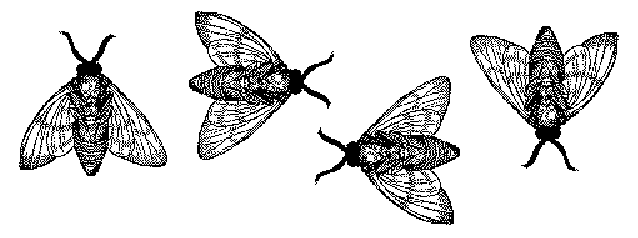
\includegraphics{flies}
\caption{A sample black and white graphic (.pdf format)
that needs to span two columns of text.}
\label{fig:flies}
\end{figure*}


Note that only {\textbf{.pdf}} files were used; if you want to include
{\textbf{.ps}} or {\textbf{.eps}} formats, you can use the
\texttt{{\char'134}epsfig} or \texttt{{\char'134}psfig}
commands as appropriate for the different file types.

\subsection{Theorem-like Constructs}
Other common constructs that may occur in your article are
the forms for logical constructs like theorems, axioms,
corollaries and proofs.  There are
two forms, one produced by the
command \texttt{{\char'134}newtheorem} and the
other by the command \texttt{{\char'134}newdef}; perhaps
the clearest and easiest way to distinguish them is
to compare the two in the output of this sample document:

This uses the \textbf{theorem} environment, created by
the\linebreak\texttt{{\char'134}newtheorem} command:
\newtheorem{theorem}{Theorem}
\begin{theorem}
Let $f$ be continuous on $[a,b]$.  If $G$ is
an antiderivative for $f$ on $[a,b]$, then
\begin{displaymath}\int^b_af(t)dt = G(b) - G(a).\end{displaymath}
\end{theorem}

The other uses the \textbf{definition} environment, created
by the \texttt{{\char'134}newdef} command:
\newdef{definition}{Definition}
\begin{definition}
If $z$ is irrational, then by $e^z$ we mean the
unique number which has
logarithm $z$: \begin{displaymath}{\log e^z = z}\end{displaymath}
\end{definition}

Two lists of constructs that use one of these
forms is given in the
\textit{Author's  Guidelines}.


There is one other similar construct environment, which is
already set up
for you; i.e. you must \textit{not} use
a \texttt{{\char'134}newdef} command to
create it: the \textbf{proof} environment.  Here
is a example of its use:
\begin{proof}
Suppose on the contrary there exists a real number $L$ such that
\begin{displaymath}
\lim_{x\rightarrow\infty} \frac{f(x)}{g(x)} = L.
\end{displaymath}
Then
\begin{align*}
l&=\lim_{x\rightarrow c} f(x)
= \lim_{x\rightarrow c}
\left[ g{x} \cdot \frac{f(x)}{g(x)} \right ] \\
&= \lim_{x\rightarrow c} g(x) \cdot \lim_{x\rightarrow c}
\frac{f(x)}{g(x)} = 0\cdot L = 0,
\end{align*}
which contradicts our assumption that $l\neq 0$.
\end{proof}

Complete rules about using these environments and using the
two different creation commands are in the
\textit{Author's Guide}; please consult it for more
detailed instructions.  If you need to use another construct,
not listed therein, which you want to have the same
formatting as the Theorem
or the Definition\cite{salas:calculus} shown above,
use the \texttt{{\char'134}newtheorem} or the
\texttt{{\char'134}newdef} command,
respectively, to create it.

\subsection*{A {\secit Caveat} for the \TeX\ Expert}
Because you have just been given permission to
use the \texttt{{\char'134}newdef} command to create a
new form, you might think you can
use \TeX's \texttt{{\char'134}def} to create a
new command: \textit{Please refrain from doing this!}
Remember that your \LaTeX\ source code is primarily intended
to create camera-ready copy, but may be converted
to other forms -- e.g. HTML. If you inadvertently omit
some or all of the \texttt{{\char'134}def}s recompilation will
be, to say the least, problematic.

\section{Conclusions}
This paragraph will end the body of this sample document.
Remember that you might still have Acknowledgments or
Appendices; brief samples of these
follow.  There is still the Bibliography to deal with; and
we will make a disclaimer about that here: with the exception
of the reference to the \LaTeX\ book, the citations in
this paper are to articles which have nothing to
do with the present subject and are used as
examples only.
%\end{document}  % This is where a 'short' article might terminate

% ensure same length columns on last page (might need two sub-sequent latex runs)
\balance

%ACKNOWLEDGMENTS are optional
\section{Acknowledgments}
This section is optional; it is a location for you
to acknowledge grants, funding, editing assistance and
what have you.  In the present case, for example, the
authors would like to thank Gerald Murray of ACM for
his help in codifying this \textit{Author's Guide}
and the \textbf{.cls} and \textbf{.tex} files that it describes.


% The following two commands are all you need in the
% initial runs of your .tex file to
% produce the bibliography for the citations in your paper.
\bibliographystyle{abbrv}
\bibliography{vldb_sample}  % vldb_sample.bib is the name of the Bibliography in this case
% You must have a proper ".bib" file
%  and remember to run:
% latex bibtex latex latex
% to resolve all references

\subsection{References}
Generated by bibtex from your ~.bib file.  Run latex,
then bibtex, then latex twice (to resolve references).

%APPENDIX is optional.
% ****************** APPENDIX **************************************
% Example of an appendix; typically would start on a new page
%pagebreak

\begin{appendix}
You can use an appendix for optional proofs or details of your evaluation which are not absolutely necessary to the core understanding of your paper. 

\section{Final Thoughts on Good Layout}
Please use readable font sizes in the figures and graphs. Avoid tempering with the correct border values, and the spacing (and format) of both text and captions of the PVLDB format (e.g. captions are bold).

At the end, please check for an overall pleasant layout, e.g. by ensuring a readable and logical positioning of any floating figures and tables. Please also check for any line overflows, which are only allowed in extraordinary circumstances (such as wide formulas or URLs where a line wrap would be counterintuitive).

Use the \texttt{balance} package together with a \texttt{\char'134 balance} command at the end of your document to ensure that the last page has balanced (i.e. same length) columns.

\end{appendix}



\end{document}
